\shorthandoff{"}
\chapter{Person-Environment Fit}
\label{ch:personEnvironmentFit}

\section{Einführung}
\label{ch:personEnvironmentFit:einfuehrung}
Der \acf{PEFit} ist ein Konzept, welches häufig im Kontext der Berufs- und Organisationspsychologie Anwendung findet \cite[S. 2]{guan:2021}. In manchen Publikationen existiert die Theorie auch unter ähnlichen Bezeichnungen mit derselben Bedeutung wie Person-Environment Korrespondenz \cite[S. 1]{eggerth:2008} oder -Kongruenz \cite[S. 1]{muchinsky:1987}\cite[S. 53]{edwards:2008}\cite[S. 3]{edwards:2007}. Es enthält drei zentrale Größen: Person, Umgebung (Environment) und Ergebnis \cite[S. 2]{livingstone:1997}.

\textcite[S. 5]{edwards:2007} stellten fest, dass die Literatur unter der Person ein menschliches Individuum versteht. Umgebung und Ergebnis werden ihren Beobachtungen zu Folge dagegen als breite Terminologien interpretiert und je nach Forschungsdomäne genauer spezifiziert \cite[S. 1ff.]{edwards:2007}. Beispiele für Ergebnisse sind Zufriedenheit \cite[S. 1]{lashani:2021}, Wechselbereitschaft \cite[S. 1]{amarneh:2021}, Kreativität \cite[S. 1]{duan:2019}, Leistung \cite[S. 6ff.]{elfenbein:2007} und  Berufswahl \cite[S. 1]{cable:1996}\cite[S. 1]{edwards:2007}. Als Umgebung untersuchten verschiedene Publikationen unter anderem Unternehmen \cite[S. 1]{kristof:1996}, Gruppen \cite[S. 1]{werbel:2001} und Arbeitsplätze \cite[S. 1]{lu:2014}\cite[S. 5]{edwards:2007}.

Die Wissenschaft geht davon aus, dass ein Ergebnis stets vom Zusammenspiel von Person und Umgebung abhängig ist und nicht durch eine der beiden Größen alleine bestimmt wird \cite[S. 1f.]{muchinsky:1987}. Wie in Abbildung \ref{fig:personEnvironmentFit:einfuehrung:abb1} verdeutlicht, ist der Fit somit selbst kein Ergebnis, sondern eine unabhängige Variable, welche zur Vorhersage eines untersuchten Resultates herangezogen wird \cite[S. 11]{caplan:1993}\cite[S.5]{edwards:1991}\cite[S. 1]{edwards:2002}.

\begin{figure}[h]
	\centering
	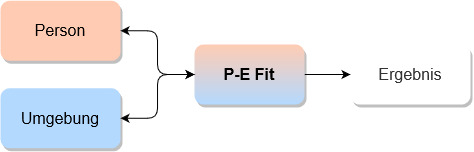
\includegraphics[width=1\textwidth]{gfx/P-E Fit.jpg}
	\caption{Zusammenwirken von Person, Umgebung, \acs{PEFit} und Ergebnis}
	\label{fig:personEnvironmentFit:einfuehrung:abb1}
\end{figure}

Der in Abbildung \ref{fig:personEnvironmentFit:einfuehrung:abb1} dargestellte \ac{PEFit} gibt an, zu welchem Grad sich die untersuchten Werte von Person und Umgebung auf einem Niveau befinden \cite[S. 53]{edwards:2008}. Dabei wird der Fit häufig nicht als Zustand, sondern als wechselseitiger Prozess betrachtet, in dem Person und Umgebung miteinander interagieren und sich dabei gegenseitig verändern \cite[S. 10ff.]{su:2015}. Diese Modifikationen können die Kongruenz sowohl verbessern als auch verschlechtern \cite[S. 4]{caplan:1987}. Aus diesem Grund können Unternehmen auch Maßnahmen ergreifen, welche den \ac{PEFit} gezielt optimieren \cite[S. 16]{cable:2001}.

\textcite[S. 6ff.]{edwards:2007} unterschieden drei Ebenen, auf welchen ein Fit bestimmbar ist. Die oberste bezeichneten sie als globale Ebene. Hier werden Person und Umgebung als Ganzes ohne weitere Untergliederungen miteinander vergleichen. Von der Domänen-Ebene sprachen \textcite[S. 7f.]{edwards:2007}, wenn eine Einteilung in mehrere sehr breite Bereiche vorgenommen wird, welche stellvertretend für Person und Umgebung miteinander vergleichen werden. Domänen können den Autoren zu Folge beispielsweise Werte, Bildung oder Berufserfahrung sein. Findet die Untersuchung ausschließlich innerhalb einer Domäne statt, bezeichneten \textcite[S. 7f.]{edwards:2007} dies als Facetten-Ebene. Als Beispiel nannten sie die Bestimmung eines \acp{PEFit} hinsichtlich demographischer Ähnlichkeit anhand von Dimensionen wie Alter und Bildung.

Wie die Kongruenz von Person und Umgebung bestimmt wird, ist von der konkreten Art des Fits abhängig. \textcite[S. 1]{muchinsky:1987} unterschieden zwischen ergänzendem und komplementärem Fit.

\section{Ergänzender und komplementärer Fit}
\label{ch:personEnvironmentFit:supplementaryUndComplementary}
Ein ergänzender Fit entsteht, wenn Person und Umgebung gleiche Werte und Interessen aufweisen \cite[S. 2ff.]{muchinsky:1987}. Diese Art der Kongruenz ist laut \textcite[S. 5ff.]{schneider:1987} ein entscheidender Faktor, von welchen Unternehmen sich potentielle Arbeitnehmer angezogen fühlen und welche Bewerber von Betrieben eingestellt werden. \textcite[S. 4, Z. 47f.]{popovich:1982} zu Folge kann der Beitritt einer Person zu einem Unternehmen sogar als ein "sehr konkreter, öffentlicher Ausdruck der Werte"\footnote{"a very concrete, public expression of values" - \textcite[S. 4, Z. 47f.]{popovich:1982}} eines Individuums interpretiert werden.

Verschiedene Autoren diskutierten die Ergebnisse des ergänzenden Fits in der Literatur kontrovers. \textcite[S. 6]{schneider:1987} stellte fest, dass Angestellte mit einer geringen Übereinstimmung ihrer Werte eher dazu tendieren, das Unternehmen zu verlassen. So entsteht dem Autor zu Folge im Betrieb langfristig eine hohe Homogenität innerhalb der Belegschaft. Diese äußert sich einerseits in positiven Ergebnissen wie einer ausgeprägten Arbeitszufriedenheit und einer starken Identifikation mit dem Unternehmen \cite[S. 26]{kristof:1996}. Die mangelnde Diversität führt aber anderseits auch zu negativen Folgen wie einer geringeren Fähigkeit zu Veränderungen \cite[S. 10]{schneider:1987} und verminderter Kreativität \cite[S. 7]{chatman:1998} und Innovation im Unternehmen \cite[S. 11]{chatman:1989}. \cite[S. 4]{su:2015}

Wenn sich Person und Umgebung nicht ähneln, sondern gegenseitig vervollständigen, sprachen \textcite[S. 4]{muchinsky:1987} vom komplementären Fit. Dabei gleichen Person und Umgebung den Autoren zu Folge Schwächen des anderen durch eigene Stärken aus.

Die komplementäre Kongruenz wird, wie in Abbildung \ref{fig:personEnvironmentFit:supplementaryUndComplementary:abb1} dargestellt, in zwei weitere Fits untergliedert. Bei dieser Betrachtungsweise haben Person und Umgebung je eine Angebots- und eine Nachfrageperspektive. Die Nachfrage der einen Partei wird dabei durch das Angebot der anderen erfüllt. \cite[S. 2ff.]{caplan:1987}\cite[S. 2ff.]{edwards:1991}\cite[S. 2]{copingAndAdaption:1974}\cite[S. 3f.]{kristof:1996}

\begin{figure}[h]
	\centering
	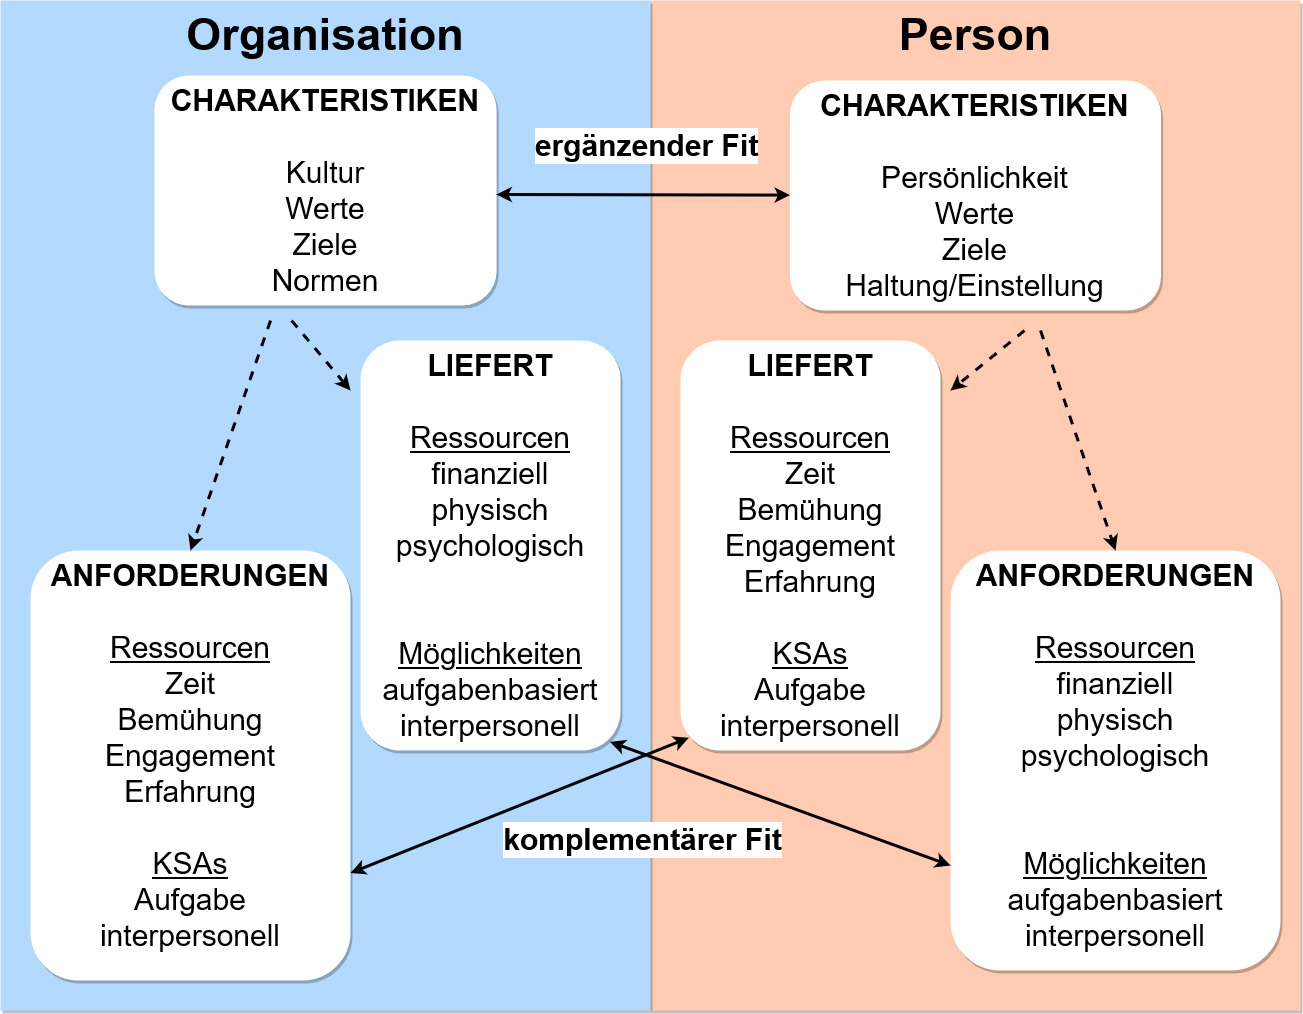
\includegraphics[width=1\textwidth]{gfx/supplementaryComplementaryFit.jpg}
	\caption[Ergänzender und komplementärer \acs{PEFit}]{Ergänzender und komplementärer \acs{PEFit}\\
	(Eigene Darstellung in Anlehnung an \cite[S. 4]{kristof:1996})}
	\label{fig:personEnvironmentFit:supplementaryUndComplementary:abb1}
\end{figure}

Unter der in Abbildung \ref{fig:personEnvironmentFit:supplementaryUndComplementary:abb1} dargestellten Nachfrage der Umgebung werden Anforderungen an die Person zusammengefasst. Hierzu zählen beispielsweise Rollen- und Leistungserwartungen. Das entsprechende Angebot der Person umfasst Fähigkeiten, Fertigkeiten, Wissen, Bildung und Arbeitserfahrung. Gleichen sich Nachfrage der Umgebung und Angebot der Person gegenseitig aus, entsteht der Anforderungen-Fähigkeiten Fit. Dieser resultiert in einer hohen Leistung und Effizienz von Individuum und Umgebung. \cite[S. 3f.]{edwards:1991}\cite[S. 5f.]{edwards:1996}\cite[S. 4]{edwards:2007}\cite[S. 7]{su:2015}

Die Nachfrage der Person in Abbildung \ref{fig:personEnvironmentFit:supplementaryUndComplementary:abb1} entspricht ihren psychologischen Bedürfnissen. Dazu zählen persönliche Präferenzen, Interessen, Motive und Ziele. Die entsprechenden Angebote der Umgebung umfassen Ressourcen und Belohnungen wie Gehalt und Mitbestimmungsrechte, welche die Bedürfnisse des Individuums befriedigen. Sind Nachfrage der Person und Angebot der Umgebung gleich stark ausgeprägt, wird dies in der Literatur als Bedürfnisse-Angebote Fit bezeichnet. Dieser resultiert in einem hohen Wohlbefinden des Mitarbeiters, welches sich beispielsweise in Zufriedenheit und verminderter Wechselbereitschaft äußert. \cite[S. 2]{edwards:2004}\cite[S. 2f.]{edwards:1996}\cite[S. 4]{edwards:2008}\cite[S. 4f.]{edwards:2007}\cite[S. 7]{su:2015}

Laut \textcite[S. 9ff.]{workAdjustment:1964} führen unausgeglichene Nachfragen langfristig zu einem Wechsel des Arbeitsplatzes. Die Autoren betrachteten die aus unzureichend erfüllten Anforderungen des Unternehmens entstehende mangelnde Arbeitsleistung als Ursache für Kündigung oder Versetzung des Mitarbeiters seitens des Arbeitgebers. Die Unzufriedenheit, welche aus unzureichend erfüllten Bedürfnissen des Angestellten resultiert, bezeichneten sie als einen Wechselgrund seitens des Mitarbeiters.

\textcite[S. 1, Z. 2]{edwards:2004} charakterisierten ergänzende und komplementäre Kongruenz als "parallele, aber unterschiedliche Strömungen"\footnote{"parallel but separate streams" - \textcite[S. 1, Z. 2]{edwards:2004}} innerhalb der \ac{PEFit}-Forschung. Doch sie stellten fest, dass beide Fits nicht vollkommen unabhängig voneinander sind. Die Ursache sahen sie in den inneren Werten von Person und Umgebung. Diese sind den Autoren zu Folge einerseits ausschlaggebend für den ergänzenden Fit, beeinflussen aber auch stark die Bedürfnisse der Person und die Angebote der Umgebung \cite[S. 3]{edwards:2004}. Beispielsweise könnte sich ein Individuum mit ausgeprägten familiären Werten aufgrund des ergänzenden Fits stark zu Betrieben mit einer gemeinschaftlichen Unternehmenskultur angezogen fühlen. Gleichzeitig prägt die Person aufgrund ihrer inneren Werte im komplementären Fit das Bedürfnis nach familiären Reizen wie gemeinsamen Veranstaltungen aus. Da das Unternehmen dieselben Eigenschaften besitzt, wird es eher dazu tendieren, seinen Mitarbeitern die Teilnahme an solchen Ereignissen anzubieten.

Dass der Abgleich der Charakteristiken von Person und Umgebung sehr bedeutsam für Zufriedenheit und Produktivität ist, erkannten Psychologen bereits vor über einhundert Jahren \cite[S. 3ff.]{parsons:1909}. Die Wurzeln des \acp{PEFit} reichen zurück bis ins Jahr 1909 \cite[S. 1]{su:2015}.

\section{Historische Entwicklung}
\label{ch:personEnvironmentFit:historisches}
Zu Beginn des 20. Jahrhunderts beschäftigten sich Wissenschaftler und Psychologen in zahlreichen Ländern der westlichen Welt intensiv mit dem Thema der Personalauswahl \cite[S. 1f.]{salgado:2001}. Ein Hauptanliegen der Forscher war es, individuelle Unterschiede zwischen den Menschen anzuerkennen \cite[S. 1ff.]{stern:1900}. Deren Ansichten zu Folge würde die gesamte Gesellschaft effizienter arbeiten, wenn Männer eine zu ihren wissenschaftlich ermittelten Fähigkeiten passende Tätigkeit aufnehmen würden \cite[S. 1f.]{kevles:1968}. Im Zuge dieser Entwicklungen konzipierte der Bostoner Professor Frank Parsons eine Vorgehensweise zur Berufsfindung, welche im Jahr 1909 vorgestellt wurde \cite[S. 3]{porfeli:2009}\cite[S. 1]{su:2015}. \textcite[S. 5ff.]{parsons:1909} erkannte schon zum damaligen Zeitpunkt, dass die Beziehung zwischen eigenen Fähigkeiten und Anforderungen des Berufsumfeldes eine wichtige Ursache für Effizienz, Produktqualität und Bezahlung waren. Aus diesem Grund empfahl er jungen Männern vor der Berufswahl zunächst ihre eigenen Fähigkeiten, die Anforderungen verschiedener Arbeitsplätze und die Beziehung zwischen beiden Seiten zu verstehen. Erst wenn sie diese Punkte unter Beaufsichtigung eines Berufsberaters und durch Verwendung verschiedener wissenschaftlicher Tests erfüllen, können sie sich dem Autor zu Folge für einen passenden Beruf entscheiden \cite[S. 5ff.]{parsons:1909}. Heute gilt Parsons aufgrund dieser Gedanken als "Gründungsvater der Berufsberatung"\footnote{"founding father of vocational guidance" - \textcite[S. 3, Z. 29]{porfeli:2009}} \cite[S. 3, Z. 29]{porfeli:2009} und als wichtiger Vorläufer des \acp{PEFit} \cite[S. 2]{edwards:2008}\cite[S. 1]{su:2015}.

Zum damaligen Zeitpunkt begegnete die Bevölkerung den neuartigen psychologischen Tests zunächst mit Skepsis \cite[S. 2]{kevles:1968}. Das änderte sich insbesondere im Jahr 1917 mit dem Eintritt der Vereinigten Staaten in den Ersten Weltkrieg. Das U.S. Militär stand vor der Herausforderung, innerhalb kürzester Zeit Millionen Männer in die verschiedenen spezialisierten Rollen des technisierten Krieges einzuordnen. Zu diesem Anlass setzten Wissenschaftler erstmals im großen Stil psychologische Tests zur Zuweisung von Personen zu passenden Militärpositionen ein \cite[S. 2ff.]{kevles:1968}. 

Nach dem Ersten Weltkrieg entstanden insbesondere in den 1930er-Jahren durch die Arbeiten von Kurt Lewin und Henry Murray weitere bedeutende Entwicklungen für die Entstehung des \acp{PEFit} \cite[S. 1]{edwards:1990}\cite[S. 5]{caplan:1993}. \textcite[S. 11f.]{lewin:1936} stellte fest, dass das Verhalten eines Menschen nicht nur durch das Individuum selbst, sondern durch das Zusammenspiel von Person und Umgebung zu erklären ist. Ergänzend zu diesen Erkenntnissen erarbeitete Murray sein Need-Press-Modell \cite[S. 2]{edwards:2008}. Der Wissenschaftler ging davon aus, dass jeder Mensch im Laufe seines Lebens verschiedene Bedürfnisse (Needs) unterschiedlich stark ausprägt. Diese treffen je nach Umgebung auf diverse Reize. Murray stellte fest, dass manche Reize mit bestimmten Bedürfnissen kompatibel sind. Trifft ein passendes Bedürfnis-Reiz-Paar aufeinander, entsteht Druck (Press). Personen interpretieren diesen subjektiv als schädliche oder nützliche Situation und zeigen dem Autor zu Folge eine entsprechende Reaktion \cite[S. 38ff.]{murray:1938}. Dieses Zusammenspiel von Bedürfnissen einer Person und Reizen der Umgebung entspricht der späteren Vorstellung des Bedürfnisse-Angebote Fits \cite[S. 8]{edwards:2008}. 

Die Erkenntnisse von Lewin und Murray gelten als wichtiger Grundstein für die Arbeiten verschiedener Forschungsgruppen rund um John R. P. French, Jr. \cite[S. 5]{caplan:1993}. Der Psychologe stellte im Jahr 1963 an der Universität in Michigan ein groß angelegtes Forschungsprogramm vor, in welchem Experten unterschiedlicher Fachrichtungen eng zusammenarbeiteten. Diese machten es sich zum Ziel, die Auswirkungen des sozialen Umfeldes in Industrieunternehmen auf die Gesundheit der Mitarbeiter zu untersuchen \cite[S. 1ff.]{french:1963}. Aus dieser Kollaboration entstanden wesentliche Beiträge zur Entstehung des \acp{PEFit} \cite[S. 4ff.]{caplan:1993}. Hierbei unterschieden die Forscher zwischen objektivem und subjektivem Fit \cite[S. 4f.]{caplan:1993}\cite[S. 1ff.]{copingAndAdaption:1974}\cite[S. 1ff.]{french:1966}.

\section{Objektiver und subjektiver P-E Fit}
\label{ch:personEnvironmentFit:subjektivObjektiv}
Wie in Abbildung \ref{fig:personEnvironmentFit:subjektivObjektiv:abb1} dargestellt, gingen \textcite[S. 1ff.]{copingAndAdaption:1974} davon aus, dass von Person und Umgebung je eine objektiv messbare und eine vom Individuum subjektiv wahrgenommene Version existieren.

\begin{figure}[h]
	\centering
	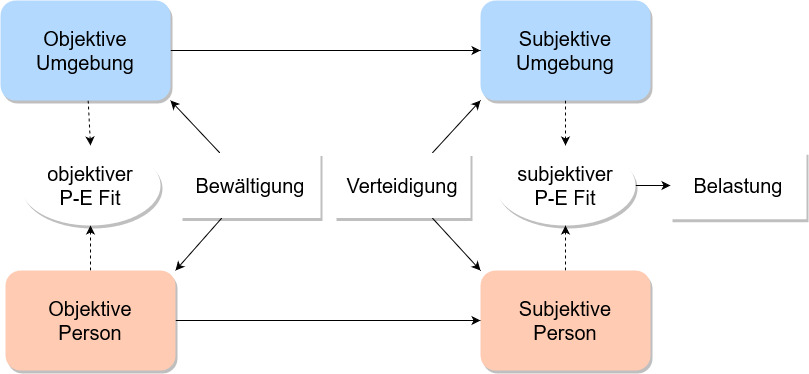
\includegraphics[width=1\textwidth]{gfx/subjektivObjektivPEFit.jpg}
	\caption[Objektiver und subjektiver \acs{PEFit}]{Objektiver und subjektiver \acs{PEFit}\\
	(Eigene Darstellung in Anlehnung an \cite[S. 2]{harrison:1978})}
	\label{fig:personEnvironmentFit:subjektivObjektiv:abb1}
\end{figure}

In der Literatur wird insbesondere der in Abbildung \ref{fig:personEnvironmentFit:subjektivObjektiv:abb1} dargestellte subjektive \ac{PEFit} als bedeutsam für die Entstehung psychischer Belastungen eingestuft und dementsprechend in der Forschung stärker fokussiert \cite[S. 8]{caplan:1987}\cite[S. 9]{caplan:1993}\cite[S. 3]{carless:2005}\cite[S. 8f.]{su:2015}.

In einer auf den Erkenntnissen von French Jr., Rodergs und Cobb aufbauenden Arbeit kam \textcite[S. 5ff.]{harrison:1978} sogar zu der Einschätzung, dass innerhalb des subjektiven \acp{PEFit} alleine die Bedürfnisse-Angebote Kongruenz Auswirkungen auf die mentale Gesundheit des Mitarbeiters hat. Ein Ungleichgewicht im Anforderungen-Fähigkeiten Fit führt dem Autor zu Folge dagegen nur dann zu psychischer Belastung, wenn diese der Erfüllung des Bedürfnisse-Angebote Fits schadet. Als Beispiel nannte der Forscher eine mit der Erfüllung einer Aufgabe verbundene Gehaltsauszahlung. Reichen die Fähigkeiten des Mitarbeiters nicht aus, die Anforderungen zu erfüllen, könnte dessen Stressgefühl zunehmen. Die Ursache für die psychische Belastung ist laut \textcite[S. 7f.]{harrison:1978} jedoch nicht das unterschiedliche Niveau von Fähigkeiten und Anforderungen, sondern die nicht erreichte Gehaltsauszahlung, welche sich der Mitarbeiter wünschte. Somit löste das Ungleichgewicht im Anforderungen-Fähigkeiten Fit nur Stress bei dem Angestellten aus, da die daraus resultierende Nichterfüllung der Aufgabe den Bedürfnisse-Angebote Fit ins Ungleichgewicht brachte.

Ein unausgewogener \ac{PEFit} wird häufig auch als Misfit bezeichnet \cite[S. 2]{edwards:2004}\cite[S. 28]{mechanismsOfJobStressAndStrain:1982}\cite[S. 4]{kristof:1996}. Mögliche Auswirkungen von P-E Misfits wurden in der Literatur in verschiedenen Arbeiten diskutiert \cite[S. 5f.]{caplan:1987}\cite[S. 21ff.]{edwards:2008}\cite[S. 28ff.]{mechanismsOfJobStressAndStrain:1982}\cite[S. 4ff.]{copingAndAdaption:1974}\cite[S. 9ff.]{harrison:1978}.

\section{Auswirkungen von P-E Misfits}
\label{ch:personEnvironmentFit:auswirkungenErhoehterAngebote}
%\textcite[S. 4ff.]{caplan:1980} stellten fest, dass ein Bedürfnisse-Angebote Misfit in unterschiedlichen Konsequenzen resultieren kann. Diese sind in Abbildung \ref{fig:personEnvironmentFit:auswirkungenErhoehterAngebote:abb1} dargestellt.
Ein Bedürfnisse-Angebote Misfit kann in drei unterschiedlichen Konsequenzen resultieren \cite[S. 21ff.]{edwards:2008}\cite[S. 28ff.]{mechanismsOfJobStressAndStrain:1982}\cite[S. 9ff.]{harrison:1978}. Diese sind in Abbildung \ref{fig:personEnvironmentFit:auswirkungenErhoehterAngebote:abb1} dargestellt.

\begin{figure}[h]
	\centering
	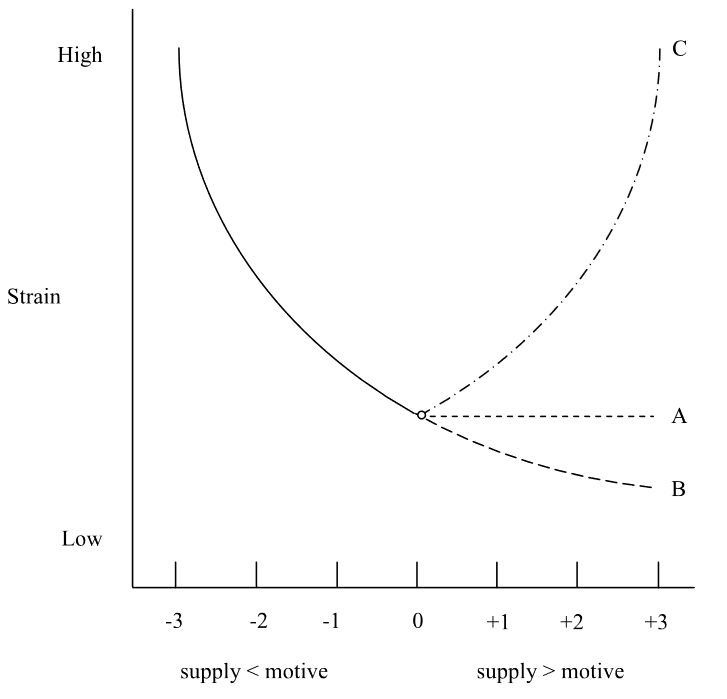
\includegraphics[width=0.75\textwidth]{gfx/ueberschuss_supply_motive.png}
	\caption[Mögliche Auswirkungen eines P-E Misfits auf die Belastung des Mitarbeiters]{Mögliche Auswirkungen eines P-E Misfits auf die Belastung des Mitarbeiters (Eigene Darstellung in Anlehnung an \cite[S. 23]{edwards:2008})}
	\label{fig:personEnvironmentFit:auswirkungenErhoehterAngebote:abb1}
\end{figure}

Die durchgezogene Linie auf der linken Hälfte von Abbildung \ref{fig:personEnvironmentFit:auswirkungenErhoehterAngebote:abb1} verdeutlicht, dass die mentale Belastung eines Individuums umso stärker zunimmt, je weniger dessen Bedürfnisse erfüllt werden \cite[S. 30]{mechanismsOfJobStressAndStrain:1982}\cite[S. 10]{harrison:1978}. Der Verlauf dieser Kurve kann über die in Gleichung \ref{fig:personEnvironmentFit:auswirkungenErhoehterAngebote:formel1} dargestellte algebraische Differenzberechnung bestimmt werden \cite[S. 2]{edwards:1993}.
\begin{equation}
	B = E - P
	\label{fig:personEnvironmentFit:auswirkungenErhoehterAngebote:formel1}
\end{equation}
Alternativ bietet sich die Verwendung der quadrierten Differenz aus Gleichung \ref{fig:personEnvironmentFit:auswirkungenErhoehterAngebote:formel3} an \cite[S. 2]{edwards:1993}.
\begin{equation}
	B = (E - P)^2
	\label{fig:personEnvironmentFit:auswirkungenErhoehterAngebote:formel3}
\end{equation}
In den Gleichungen \ref{fig:personEnvironmentFit:auswirkungenErhoehterAngebote:formel1} und \ref{fig:personEnvironmentFit:auswirkungenErhoehterAngebote:formel3} steht steht $B$ für die mentale Belastung des Mitarbeiters. $P$ stellt die von einer Person gewünschte Menge eines bestimmten Wertes dar. Die vom Mitarbeiter wahrgenommene erhaltene Menge des entsprechenden Wertes seitens der Umgebung wird über Parameter $E$ ausgedrückt. \cite[S. 1f.]{edwards:1993}\cite[S. 2ff.]{copingAndAdaption:1974}

Übersteigen die Angebote der Umgebung die Bedürfnisse der Person, mündet dies in Abbildung \ref{fig:personEnvironmentFit:auswirkungenErhoehterAngebote:abb1} in einer der drei gepunkteten Linien A, B oder C \cite[S. 29ff.]{mechanismsOfJobStressAndStrain:1982}. Kurve A zeigt einen monotonen Verlauf der mentalen Belastung. Dieser entsteht, wenn eine Person die Übererfüllung eines Bedürfnisses entweder für einen späteren Zeitpunkt aufsparen oder in die Befriedigung weiterer Motive investieren kann \cite[S. 21]{edwards:2008}\cite[S. 30]{mechanismsOfJobStressAndStrain:1982}\cite[S. 11]{harrison:1978}. Dieser Sachverhalt ist laut \textcite[S. 21]{edwards:2008} beispielsweise erfüllt, wenn einer Person mehr Gehalt zusteht, als diese für die Zahlung ihrer Lebenshaltungskosten benötigt. Dem Forscher zu Folge könnte das überschüssige Geld entweder für die Zahlung von Lebenshaltungskosten in den Folgemonaten aufgespart oder zusätzlich in das mögliche Bedürfnis nach Luxusgütern investiert werden. Für die Berechnung von Linie A kann ebenfalls Gleichung \ref{fig:personEnvironmentFit:auswirkungenErhoehterAngebote:formel1} verwendet werden \cite[S. 2]{edwards:1993}.

Kurve B hat den Verlauf einer quadratischen Funktion und tritt ein, wenn die Übererfüllung eines Bedürfnisses entweder die Befriedigung dieses oder eines verwandten Motivs hemmt \cite[S. 5]{caplan:1987}\cite[S. 21]{edwards:2008}. \textcite[S. 12]{harrison:1978} nannte hierfür das Bedürfnis einer Person nach Privatsphäre als Beispiel, welches bei Übererfüllung das Verlangen nach sozialen Beziehungen verletzt. Der Verlauf von Linie B kann über Gleichung \ref{fig:personEnvironmentFit:auswirkungenErhoehterAngebote:formel3} oder die in Gleichung \ref{fig:personEnvironmentFit:auswirkungenErhoehterAngebote:formel2} dargestellte absolute Differenzberechnung bestimmt werden \cite[S. 2]{edwards:1993}.
\begin{equation}
	B = |E - P|
	\label{fig:personEnvironmentFit:auswirkungenErhoehterAngebote:formel2}
\end{equation}
Kurve C stellt eine asymptotische Beziehung zur mentalen Belastung dar. Sie tritt ein, wenn weder die Bedingungen von Linie A noch von Kurve B zutreffen. Eine Übererfüllung des Bedürfnisses hat folglich weder positive noch negative Auswirkungen auf die Person \cite[S. 21]{edwards:2008}\cite[S. 30]{mechanismsOfJobStressAndStrain:1982}. Ein Beispiel für eine solche Beziehung ist ein Überangebot an Parkplätzen beim Arbeitgeber. Da der Mitarbeiter nur ein Fahrzeug besitzt, kann dieser von zusätzlichen Angeboten keinen Gebrauch machen und diese auch nicht für einen späteren Zeitpunkt aufsparen. Die zusätzlichen Parkplätze schaden auch keinem anderen Bedürfnis des Angestellten. Somit entstehen weder positive noch negative Auswirkungen auf dessen Wohlbefinden. Zur Bestimmung von Kurve C wird die Belastung gleich dem Wert null gesetzt. Dieses Vorgehen ist in Gleichung \ref{fig:personEnvironmentFit:auswirkungenErhoehterAngebote:formel4} dargestellt \cite[S. 2]{edwards:1993}.
\begin{equation}
	B = 0
	\label{fig:personEnvironmentFit:auswirkungenErhoehterAngebote:formel4}
\end{equation}
Verschiedene Autoren gehen davon aus, dass die Beziehungen aus Abbildung \ref{fig:personEnvironmentFit:auswirkungenErhoehterAngebote:abb1} auch für den Anforderungen-Fähigkeiten Fit zu erwarten sind \cite[S. 31]{mechanismsOfJobStressAndStrain:1982}\cite[S. 12f.]{harrison:1978}. Dies gilt gemäß der Erkenntnisse aus Kapitel \ref{ch:personEnvironmentFit:subjektivObjektiv} nur, wenn das Erfüllen der Anforderungen Auswirkungen auf die inneren Werte des Mitarbeiters hat \cite[S. 12f.]{harrison:1978}.

Wie an der durchgezogenen Linie auf der linken Seite von Abbildung \ref{fig:personEnvironmentFit:auswirkungenErhoehterAngebote:abb1} zu erkennen, entsteht in jedem Fall psychische Belastung, wenn die Anforderungen der Umgebung die Kenntnisse des Mitarbeiters übersteigen. Sind dagegen die Fähigkeiten des Angestellten stärker ausgeprägt als erforderlich, resultiert dies in einer der Kurven A bis C. Linie A tritt ein, wenn der Mitarbeiter seine gewonnenen Freiräume nutzen kann, um verwandte Bedürfnisse zu erfüllen. Schaden die zu niedrigen Anforderungen einem Motiv des Angestellten, entsteht Kurve B. Haben die zu hohen Fähigkeiten des Mitarbeiters weder positive noch negative Auswirkungen auf dessen Wohlbefinden, resultiert Linie C. \cite[S. 22f.]{edwards:2008}\cite[S. 12f.]{harrison:1978}

Unterschiedliche Publikationen stellten fest, dass der Verlauf der Kurven nicht alleine von den Auswirkungen der Misfits auf die Motive des Mitarbeiters abhängig ist. Zusätzlich muss beachtet werden, als wie wichtig der Angestellte die betroffenen Bedürfnisse bewertet. \cite[S. 9f.]{edwards:1996}

\section{Einbeziehung der Wichtigkeiten von Bedürfnissen}
\label{ch:personEnvironmentFit:wichtigkeiten}
%\textcite[S. 18]{locke:1969}
\textcite[S. 16]{harrison:1985} schlug vor, den \ac{PEFit} für jede untersuchte Dimension einzeln zu berechnen und die Ergebnisse jeweils mit einem Wichtigkeitswert zu multiplizieren. Diese Einschätzung teilt auch \textcite[S. 8ff.]{locke:1976}. Er gilt als einflussreicher Wissenschaftler auf dem Gebiet der Arbeitszufriedenheit \cite[S. 12]{edwards:2008}. Diese kann laut \textcite[S. 8]{locke:1969} nur entstehen, wenn Mitarbeiter das Gefühl haben, für sie als wichtig erachtete berufliche Werte durch ihre Tätigkeit zu erfüllen. Aus diesem Grund empfahl er zur Berechnung der Arbeitszufriedenheit eines Angestellten zwei Kennzahlen heranzuziehen: Die Differenz aus wahrgenommener und gewünschter Menge eines Wertes und die subjektive Wichtigkeit des Motivs \cite[S. 8ff.]{locke:1976}. Ein Beispiel für eine Multiplikation mit algebraischer Differenz ist in folgender Gleichung \ref{fig:personEnvironmentFit:wichtigkeiten:formel1} dargestellt \cite[S. 10]{locke:1976}.
\begin{equation}
	Y = b * (E - P)
	\label{fig:personEnvironmentFit:wichtigkeiten:formel1}
\end{equation}
In Gleichung \ref{fig:personEnvironmentFit:wichtigkeiten:formel1} steht $Y$ für das untersuchte Ergebnis wie beispielsweise die Arbeitszufriedenheit. $b$ stellt den subjektiven Wichtigkeitswert dar. Dieser wird mit der Differenz aus gewünschter Menge eines Wertes einer Person $P$ und wahrgenommener Menge des Wertes der Umgebung $E$ multipliziert \cite[S. 10]{locke:1976}.

Derartige Multiplikationen mit einem Differenzwert haben zur Folge, dass die in Abbildung \ref{fig:personEnvironmentFit:auswirkungenErhoehterAngebote:abb1} dargestellten Kurven mit steigender Wichtigkeit steiler werden \cite[S. 13f.]{edwards:2008}\cite[S. 9]{locke:1976}. Abbildung \ref{fig:personEnvironmentFit:wichtigkeiten:abb1} verdeutlicht die entstehenden Stauchungen durch Wichtigkeitswerte.

\begin{figure}[h]
	\centering
	
	\subfloat[Algebraische Differenz]{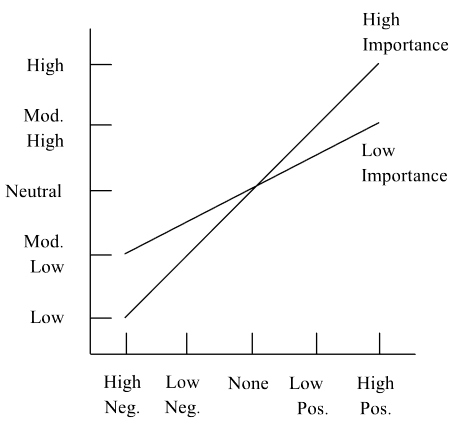
\includegraphics[width = 0.5\textwidth]{gfx/Locke-A.png}}
	\subfloat[Absolute Differenz]{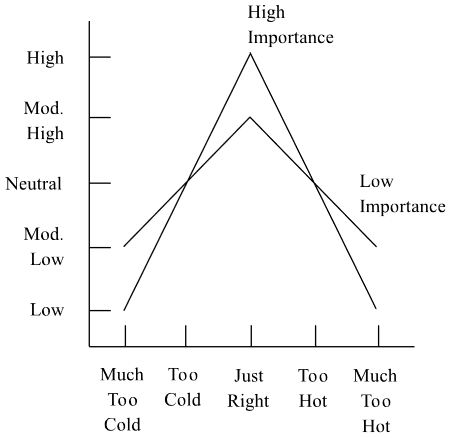
\includegraphics[width = 0.5\textwidth]{gfx/Locke-B.png}}
	
	\caption[Stauchung von Funktionsgraphen durch Wichtigkeiten]{Stauchung von Funktionsgraphen durch Wichtigkeiten\\
	(Eigene Darstellung in Anlehnung an \cite[S. 9]{locke:1976})}
	%(Aus \cite[S. 13f.]{edwards:2008}, nach \cite[S. 1305]{locke:1976})
	\label{fig:personEnvironmentFit:wichtigkeiten:abb1}
\end{figure}
\newpage
Im linken Teil (a) von Abbildung \ref{fig:personEnvironmentFit:wichtigkeiten:abb1} ist eine monotone Funktion basierend auf einer algebraischen Differenzberechnung dargestellt. Die rechte Seite der Grafik (b) zeigt den Verlauf einer Berechnung mit absoluter Differenz. In beiden Darstellungen ist zu erkennen, dass die Kurven bei fehlender Wichtigkeit ausschließlich im mittleren Bereich verlaufen. Ist einem Individuum das jeweilige Bedürfnis dagegen wichtig, füllt die Kurve den gesamten verfügbaren Bereich von niedrig bis hoch. Dieses Vorgehen führt zur Stauchung der Funktionsgraphen und damit zu einem stärkeren Ansteigen bzw. Absinken der Belastung des Individuums.

Derartige Berechnungen kritisierte \textcite[S. 51ff.]{edwards:1991}\cite[S. 9ff.]{edwards:1990}\cite[S. 2ff.]{edwards:1993}\cite[S. 2ff.]{edwards:1993b} in mehreren seiner Arbeiten. Dabei diskutierte er insbesondere die Multiplikation mit dem Differenzwert. Er ist der Auffassung, dass die aus der Differenzberechnung resultierenden zweidimensionalen Grafiken die Komplexität eines \acp{PEFit} nicht vollständig abbilden. Deshalb schlug er vor, die Berechnungen mittels Regressionsgleichungen durchzuführen \cite[S. 51ff.]{edwards:1991}\cite[S. 9ff.]{edwards:1990}\cite[S. 2ff.]{edwards:1993}\cite[S. 1ff.]{edwards:1993b}.

\section{Anwendung von Regressionsgleichungen}
\label{ch:personEnvironmentFit:regressionsgleichungen}
\textcite[S. 51ff.]{edwards:1991}\cite[S. 9ff.]{edwards:1990}\cite[S. 2ff.]{edwards:1993}\cite[S. 2ff.]{edwards:1993b} empfahl, die Multiplikationen separat für jeden Wert von Person und Umgebung durchzuführen. Formel \ref{fig:personEnvironmentFit:wichtigkeiten:formel1} könnte hierfür zu folgender Regressionsgleichung \ref{fig:personEnvironmentFit:wichtigkeiten:formel2} umgestellt werden \cite[S. 9f.]{edwards:1990}\cite[S. 2f.]{edwards:1993b}.
\begin{equation}
	Y = b_1 * E - b_2 * P + a
	\label{fig:personEnvironmentFit:wichtigkeiten:formel2}
\end{equation}
Die Koeffizienten $b_1$ und $b_2$ stehen in Gleichung \ref{fig:personEnvironmentFit:wichtigkeiten:formel2} für die separaten Wichtigkeiten von gewünschter ($P$) und wahrgenommener Menge ($E$) eines Wertes. Durch diese Art der Berechnung entstehen aus zweidimensionalen Grafiken dreidimensionale Modelle \cite[S. 2]{edwards:1993}. Solche Darstellungen sind dem Wissenschaftler zu Folge besser geeignet, Ungleichmäßigkeiten in den Oberflächen abzubilden \cite[S. 51ff.]{edwards:1991}. So stellte \textcite[S. 53ff.]{edwards:1991} bei der Datenanalyse einer Studie mit mehreren hundert Teilnehmern die in Abbildung \ref{fig:personEnvironmentFit:wichtigkeiten:abb2} dargestellte dreidimensionale Beziehung von \ac{PEFit} und Zufriedenheit fest.

\begin{figure}[h]
	\centering
	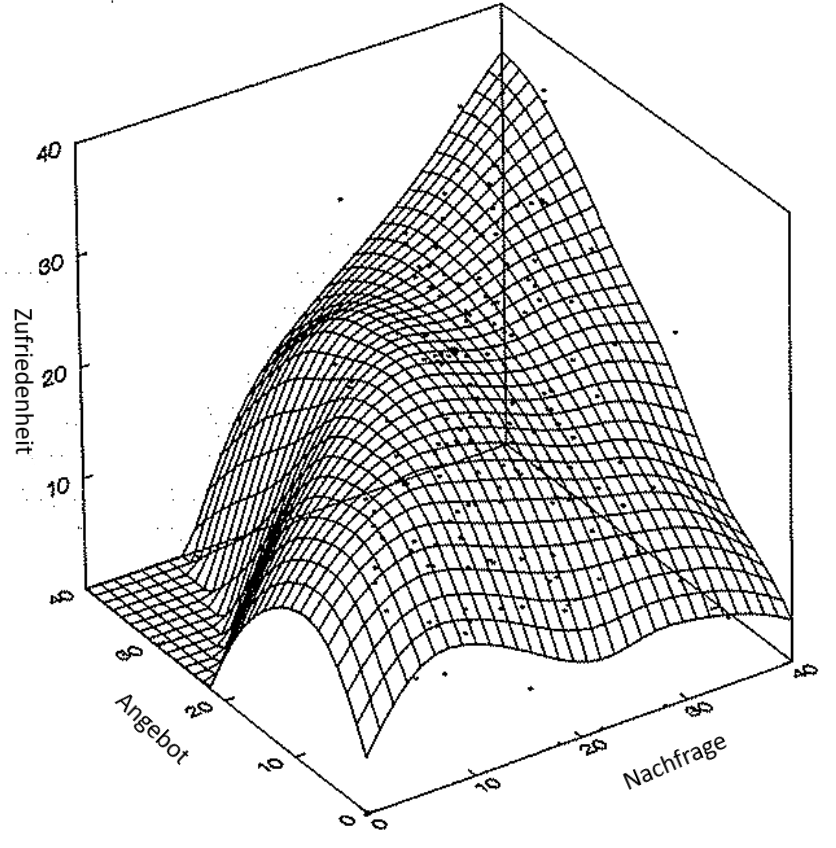
\includegraphics[width=0.8\textwidth]{gfx/drei_d_modell.png}
	\caption[Dreidimensionale Beziehung von P-E Fit und Zufriedenheit]{Dreidimensionale Beziehung von P-E Fit und Zufriedenheit\\
	(Eigene Darstellung in Anlehnung an \cite[S. 57]{edwards:1991})}
	\label{fig:personEnvironmentFit:wichtigkeiten:abb2}
\end{figure}

Um die stärkere Aussagekraft der Regressionsgleichungen zu untermauern, werteten \textcite[S. 18ff.]{edwards:1993b} einen umfangreichen Datensatz von \textcite[S. 9ff.]{mechanismsOfJobStressAndStrain:1982} erneut aus. Dabei gelang es ihnen, durch Anwendung von Regressionsgleichungen im Vergleich zur erstmaligen Untersuchung einen wesentlich höheren Anteil an Varianz zu erklären \cite[S. 8]{su:2015}.
\shorthandon{"}
